\documentclass[12pt]{article}
\usepackage{alltt}
\usepackage[utf8]{inputenc}
\usepackage[dvips]{graphicx}
%\usepackage{a4wide}
\usepackage{epsfig}
\usepackage{fancybox}
\usepackage{verbatim}
\usepackage{array}
\usepackage{latexsym}
\usepackage{alltt}
%\usepackage{dsfont}
\usepackage{caption}
\usepackage{subcaption}
%\usepackage{fullpage}
\usepackage{hyperref}
\usepackage{textcomp}
\usepackage{listings}
\usepackage{color}
\usepackage{amsmath}
\usepackage{amsfonts}
\usepackage{tikz}
\usepackage{float}
\usepackage{matlab-prettifier}
\usepackage{graphicx}

\usepackage[hmargin=3cm,vmargin=6.0cm]{geometry}

\topmargin=-1.8cm
\addtolength{\textheight}{6.5cm}
\addtolength{\textwidth}{2.0cm}
\setlength{\oddsidemargin}{0.0cm}
\setlength{\evensidemargin}{0.0cm}

\newcommand{\HRule}{\rule{\linewidth}{1mm}}

\usepackage{tikz}
\usetikzlibrary{trees}
\tikzset{
  font={\fontsize{7pt}{12}\selectfont}}
  
\newcommand{\Q}{\raisebox{1.7pt}{$\scriptstyle\bigcirc$}}

\lstset{
    %backgroundcolor=\color{lbcolor},
    tabsize=2,
    language=C++,
    basicstyle=\footnotesize,
    numberstyle=\footnotesize,
    aboveskip={0.0\baselineskip},
    belowskip={0.0\baselineskip},
    columns=fixed,
    showstringspaces=false,
    breaklines=true,
    prebreak=\raisebox{0ex}[0ex][0ex]{\ensuremath{\hookleftarrow}},
    %frame=single,
    showtabs=false,
    showspaces=false,
    showstringspaces=false,
    identifierstyle=\ttfamily,
    keywordstyle=\color[rgb]{0,0,1},
    commentstyle=\color[rgb]{0.133,0.545,0.133},
    stringstyle=\color[rgb]{0.627,0.126,0.941},
}

\usepackage[]{mdframed}
\usepackage{enumitem}

\usepackage{titlesec}
\titleformat{\subsection}[runin]{}{}{}{}[]









\begin{document}

% Set the overall layout of the tree
\tikzstyle{level 1}=[level distance=2.5cm, sibling distance=20em]
\tikzstyle{level 2}=[level distance=2.5cm, sibling distance=10em]

% Define styles for bags and leafs
\tikzstyle{bag} = [text width=16em, text centered, align=center]
\tikzstyle{end} = [circle, minimum width=3pt,fill, inner sep=0pt]

\noindent
\HRule \\[3mm]
\small
\begin{tabular}[b]{lp{4.3cm}r}
Middle East Technical University &  &
Department of Computer Engineering \\
\end{tabular} \\
\begin{center}

                 \LARGE \textbf{CENG 280} \\[4mm]
                 \Large Formal Languages and Abstract Machines \\[4mm]
                \normalsize Spring 2022-2023 \\
                    \Large Homework 6 \\
\end{center}
\HRule



% Write down your name, surname, and student ID below.
\begin{center}
Name Surname: Doruk Berke Yurtsizoglu   \\
Student ID: 2522225
\end{center}



\section*{Answer for Q1}
   
Alan Turing was born in June 23 1912 and died in June 7 1954. \\
\\
Turing played a crucial role in breaking the Enigma code during World War II. \\
\\
The now-famous Turing test , proposed in his paper Computing Machinery and Intelligence (1950), is an attempt to define a standard for a machine to be called “intelligent". \\
\\
One of his most-cited works, titled Theory of Morphogenesis was published in 1952, which proposed a mechanism as to how inhomogeneous patterns in nature arise from symmetric starting states. \\
\\
The 2014 movie titled The Immitation Game aims to give a biographical portrait of Turing. \\




\section*{Answer for Q2}

\subsection*{a.} 

The turing machine we are going to construct is going to read all a's and replaces them with the blank symbol until it finds a b. It will repeat the process once more. When it finds the second b, it will halt if and only if it reaches the end of the string. Otherwise, it will go to a trap state and will enter to an infinite loop. Also, if machine encounters a blank symbol before reaching the second b, the machine will enter the infinite loop. The turing machine that satisfies these conditions is:\\

\begin{center}
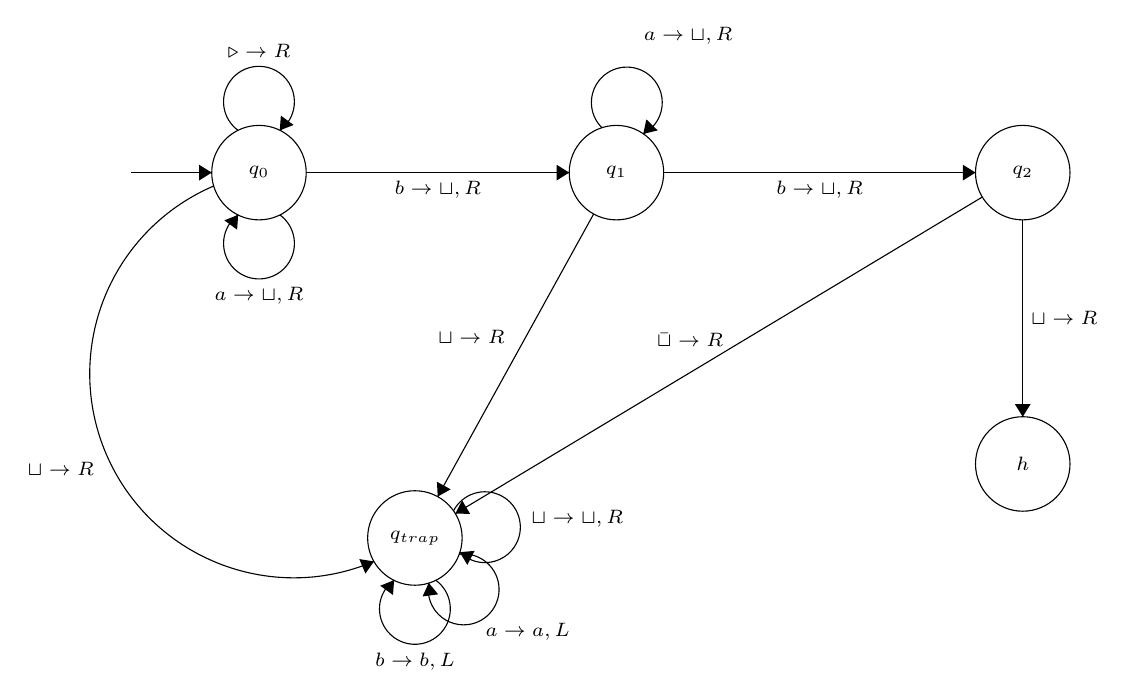
\begin{tikzpicture}[scale=0.2]
\tikzstyle{every node}+=[inner sep=0pt]
\draw [black] (13.7,-11.7) circle (3);
\draw (13.7,-11.7) node {$q_0$};
\draw [black] (36.4,-11.7) circle (3);
\draw (36.4,-11.7) node {$q_1$};
\draw [black] (62.2,-11.7) circle (3);
\draw (62.2,-11.7) node {$q_2$};
\draw [black] (62.2,-30.2) circle (3);
\draw (62.2,-30.2) node {$h$};
\draw [black] (23.6,-34.9) circle (3);
\draw (23.6,-34.9) node {$q_{trap}$};
\draw [black] (5.6,-11.7) -- (10.7,-11.7);
\fill [black] (10.7,-11.7) -- (9.9,-11.2) -- (9.9,-12.2);
\draw [black] (12.377,-9.02) arc (234:-54:2.25);
\draw (13.7,-4.45) node [above] {$\triangleright \rightarrow R$};
\fill [black] (15.02,-9.02) -- (15.9,-8.67) -- (15.09,-8.08);
\draw [black] (15.023,-14.38) arc (54:-234:2.25);
\draw (13.7,-18.95) node [below] {$a \rightarrow \sqcup,R$};
\fill [black] (12.38,-14.38) -- (11.5,-14.73) -- (12.31,-15.32);
\draw [black] (16.7,-11.7) -- (33.4,-11.7);
\fill [black] (33.4,-11.7) -- (32.6,-11.2) -- (32.6,-12.2);
\draw (25.05,-12.2) node [below] {$b \rightarrow \sqcup, R$};
\draw [black] (35.484,-8.855) arc (225.57303:-62.42697:2.25);
\draw (40.95,-3.61) node [above] {$a \rightarrow \sqcup, R$};
\fill [black] (38.1,-9.24) -- (39.02,-9.02) -- (38.3,-8.32);
\draw [black] (39.4,-11.7) -- (59.2,-11.7);
\fill [black] (59.2,-11.7) -- (58.4,-11.2) -- (58.4,-12.2);
\draw (49.3,-12.2) node [below] {$b \rightarrow \sqcup, R$};
\draw [black] (62.2,-14.7) -- (62.2,-27.2);
\fill [black] (62.2,-27.2) -- (62.7,-26.4) -- (61.7,-26.4);
\draw (62.7,-20.95) node [right] {$\sqcup \rightarrow R$};
\draw [black] (21.001,-36.386) arc (-66.87298:-246.9088:12.959);
\fill [black] (21,-36.39) -- (20.07,-36.24) -- (20.46,-37.16);
\draw (3.26,-30.5) node [left] {$\sqcup \rightarrow R$};
\draw [black] (34.95,-14.33) -- (25.05,-32.27);
\fill [black] (25.05,-32.27) -- (25.87,-31.81) -- (25,-31.33);
\draw (29.33,-22.1) node [left] {$\sqcup \rightarrow R$};
\draw [black] (59.63,-13.25) -- (26.17,-33.35);
\fill [black] (26.17,-33.35) -- (27.11,-33.37) -- (26.6,-32.51);
\draw (41.07,-22.8) node [above] {$\bar{\sqcup} \rightarrow R$}; %ha
\draw [black] (24.923,-37.58) arc (54:-234:2.25);
\draw (23.6,-42.15) node [below] {$b \rightarrow b, L$};
\fill [black] (22.28,-37.58) -- (21.4,-37.93) -- (22.21,-38.52);
\draw [black] (26.403,-35.936) arc (97.45184:-190.54816:2.25);
\draw (30.76,-40.28) node [below] {$a \rightarrow a, L$};
\fill [black] (24.48,-37.75) -- (24.09,-38.61) -- (25.08,-38.48);
\draw [black] (26.047,-33.185) arc (152.74616:-135.25384:2.25);
\draw (30.97,-33.68) node [right] {$\sqcup \rightarrow \sqcup, R$};
\fill [black] (26.45,-35.8) -- (26.93,-36.61) -- (27.39,-35.72);
\end{tikzpicture}
\end{center}

.\\
M = $(K, \sum, \delta, s, H)$\\
H = $\{ h \}$\\
K = $\{ q_0 , q_1 , q_2 , q_{trap}, h \}$\\
$\sum$ = $\{ a, b, \sqcup , \triangleright \}$\\
s = $\{ q_0 \}$\\
\\
$\delta (q_0 , \triangleright )$ = $(q_0 , \rightarrow)$\\
$\delta (q_0 , a )$ = $(q_0 , \rightarrow)$\\
$\delta (q_0 , b )$ = $(q_1 , \rightarrow)$\\
$\delta (q_0 , \sqcup )$ = $(q_{trap} , \rightarrow)$\\
\\
$\delta (q_1 , \triangleright )$ = $(q_1 , \rightarrow)$\\
$\delta (q_1 , a )$ = $(q_1 , \rightarrow)$\\
$\delta (q_1 , b )$ = $(q_2 , \rightarrow)$\\
$\delta (q_1 , \sqcup )$ = $(q_{trap} , \rightarrow)$\\
\\
$\delta (q_2 , \triangleright )$ = $(q_2 , \rightarrow)$\\
$\delta (q_2 , a )$ = $(q_{trap} , \rightarrow)$\\
$\delta (q_2 , b )$ = $(q_{trap} , \rightarrow)$\\
$\delta (q_2 , \sqcup )$ = $(h , \rightarrow)$\\
\\
$\delta (q_{trap} , \triangleright )$ = $(q_{trap} , \rightarrow)$\\
$\delta (q_{trap} , a )$ = $(q_{trap} , \leftarrow)$\\
$\delta (q_{trap} , b )$ = $(q_{trap} , \leftarrow)$\\
$\delta (q_{trap} , \sqcup )$ = $(q_{trap} , \rightarrow)$\\

\subsection*{b.} 

\begin{center}
\begin{tikzpicture}[scale=0.2]
\tikzstyle{every node}+=[inner sep=0pt]
\draw [black] (10.6,-10.6) circle (3);
\draw (10.6,-10.6) node {$R$};
\draw [black] (27.8,-10.6) circle (3);
\draw (27.8,-10.6) node {$R$};
\draw [black] (46.3,-10.6) circle (3);
\draw (46.3,-10.6) node {$R$};
\draw [black] (65.3,-10.6) circle (3);
\draw (65.3,-10.6) node {$h$};
\draw [black] (23,-29.8) circle (3);
\draw (23,-29.8) node {$L$};
\draw [black] (44.7,-29.8) circle (3);
\draw (44.7,-29.8) node {$R$};
\draw [black] (9.652,-7.766) arc (226.23483:-61.76517:2.25);
\draw (11.81,-3.32) node [above] {$a$};
\fill [black] (12.27,-8.12) -- (13.19,-7.89) -- (12.46,-7.2);
\draw [black] (13.6,-10.6) -- (24.8,-10.6);
\fill [black] (24.8,-10.6) -- (24,-10.1) -- (24,-11.1);
\draw (19.2,-11.1) node [below] {$b$};
\draw [black] (26.2,-8.076) arc (240.1155:-47.8845:2.25);
\draw (26.88,-3.31) node [above] {$a$};
\fill [black] (28.83,-7.79) -- (29.66,-7.35) -- (28.79,-6.85);
\draw [black] (30.8,-10.6) -- (43.3,-10.6);
\fill [black] (43.3,-10.6) -- (42.5,-10.1) -- (42.5,-11.1);
\draw (37.05,-11.1) node [below] {$b$};
\draw [black] (49.3,-10.6) -- (62.3,-10.6);
\fill [black] (62.3,-10.6) -- (61.5,-10.1) -- (61.5,-11.1);
\draw (55.8,-11.1) node [below] {$\sqcup$};
\draw [black] (12.23,-13.12) -- (21.37,-27.28);
\fill [black] (21.37,-27.28) -- (21.36,-26.34) -- (20.52,-26.88);
\draw (16.18,-21.51) node [left] {$\sqcup$};
\draw [black] (27.07,-13.51) -- (23.73,-26.89);
\fill [black] (23.73,-26.89) -- (24.41,-26.23) -- (23.44,-25.99);
\draw (24.64,-19.74) node [left] {$\sqcup$};
\draw [black] (43.98,-12.51) -- (25.32,-27.89);
\fill [black] (25.32,-27.89) -- (26.25,-27.77) -- (25.61,-27);
\draw (29.02,-19.71) node [above] {$\bar{\sqcup}$};
\draw [black] (25.82,-28.781) arc (106.77024:73.22976:27.829);
\fill [black] (41.88,-28.78) -- (41.26,-28.07) -- (40.97,-29.03);
\draw (33.85,-27.1) node [above] {$\sqcup$};
\draw [black] (41.786,-30.509) arc (-78.4867:-101.5133:39.759);
\fill [black] (25.91,-30.51) -- (26.6,-31.16) -- (26.8,-30.18);
\draw (33.85,-31.81) node [below] {$\sqcup$};
\draw [black] (46.023,-32.48) arc (54:-234:2.25);
\draw (44.7,-37.05) node [below] {$\bar{\sqcup}$};
\fill [black] (43.38,-32.48) -- (42.5,-32.83) -- (43.31,-33.42);
\draw [black] (24.323,-32.48) arc (54:-234:2.25);
\draw (23,-37.05) node [below] {$\bar{\sqcup}$};
\fill [black] (21.68,-32.48) -- (20.8,-32.83) -- (21.61,-33.42);
\draw [black] (2.5,-10.6) -- (7.6,-10.6);
\fill [black] (7.6,-10.6) -- (6.8,-10.1) -- (6.8,-11.1);
\end{tikzpicture}
\end{center}








\section*{Answer for Q3}

$-$ Let's assign each tape with different mission:\\
Tape 1 $\rightarrow$ input tape\\
Tape 2 $\rightarrow$ calculation tape\\
Tape 3 $\rightarrow$ result tape (initial value of this tape will be 1)\\
\\
$-$ Steps to follow for Integer Exponentiation: $(a^b)$\\
1. Read the input from Tape 1, get the values of a and b.\\
\\
2. While b is greater than 0;\\
$--$ Use the turing machine $M_x$ to multiply the value on Tape 3 with the value of a on Tape 2. Store the result to Tape 3.\\
$--$ Subtract 1 from b by using the turing $M_-$.\\
\\
3. If b is equal to 0, use $M_x$ to multiply the value on Tape 3 with 1.\\
\\
4. Write the final value of Tape 3 as the result.\\
\\
5. Halt\\  







\end{document}
